\UseRawInputEncoding
\documentclass[a4paper, 12pt]{article}

\usepackage[a4paper, margin=1in]{geometry}
\usepackage[utf8]{inputenc}
\usepackage[T1]{fontenc}

\usepackage{graphicx}
\usepackage{subcaption}
\usepackage{fancyhdr}
\usepackage{titlesec}
\usepackage{hyperref}
\usepackage{enumitem}
\usepackage{booktabs}
\usepackage{listings}
\usepackage{xcolor}
\usepackage{float}
\usepackage{tikz}
\usetikzlibrary{positioning, arrows.meta, calc, chains, fit, backgrounds}
\usepackage{bytefield}

% Header and Footer Configuration
\pagestyle{fancy}
\fancyhf{}
\fancyhead[L]{Segurança de Redes e Sistemas Distribuídos - 2026}
\fancyhead[R]{\IfFileExists{logo.png}{\includegraphics[height=1.5cm]{logo.png}}{}}
\fancyfoot[C]{\thepage}
\setlength{\headheight}{45pt}
\setlength{\headsep}{20pt}

% Section Titles Styling
\titleformat{\section}{\large\bfseries}{\thesection}{1em}{}
\titleformat{\subsection}{\normalsize\bfseries}{\thesubsection}{1em}{}

\lstset{
    basicstyle=\ttfamily\small,
    breaklines=true,
    frame=single,
    backgroundcolor=\color{gray!10},
}

\begin{document}

\begin{titlepage}
    \centering
    \IfFileExists{logo.png}{\includegraphics[width=3cm]{logo.png}\par\vspace{1cm}}{}
    \vspace*{1cm}
    {\Large \textbf{Faculdade de Ciências da Universidade de Lisboa}}\\[0.5em]
    \vspace{4cm}
    {\Huge \textbf{Secure Gallery Log System}} \\
    \vspace{1.5cm}
    {\Large \textbf{José Sampaio, fc66191}}\\[0.5em]
    {\Large \textbf{Rodrigo Neto, fc59850}}\\[0.5em]
    {\Large \textbf{Gabriel Cambraia, 58671}}\\[1em]
    \vfill

{\large Segurança de Redes e Sistemas Distribuídos}\\
{\large 2026}\par\vspace{2cm}

\end{titlepage}
\tableofcontents
\newpage

% ===========================================================================
\section{Introduction}
% ===========================================================================
For this first part of the project, we implemented two CLI tools, \texttt{logappend} and \texttt{logread}, that manage an append-only, encrypted gallery log. These tools track employee and guest arrivals and departures through a gallery and its rooms. The \texttt{logappend} tool creates a log file and appends entries to it, while \texttt{logread} allows users to query the current state of the log and perform history analysis, such as checking which rooms a person has visited or identifying rooms where people have crossed paths. The project has a strong emphasis on security: confidentiality, integrity, and authenticity are central to the design. We also aimed for an implementation that is both optimized and performant. With these goals in mind, we chose Rust as our programming language, as it enables the creation of secure, high-performance software with low-level memory management and strong safety guarantees.

% ===========================================================================
\section{System Architecture}
% ===========================================================================
\subsection{Overview}
The system consists of two CLI tools: \texttt{logappend}, which writes new events to the log after validating the full chain and gallery state machine, and \texttt{logread}, which reads and decrypts the log to answer state, room-history, and intersection queries. Both tools share a single library crate (\texttt{lib.rs}) that contains all crypto, encoding, state-machine, and query logic. The log itself is stored as a single flat binary file, with no external database or index.
\subsection{Threat Model}
We assume the adversary has full read/write access to the log file on disk but does \emph{not} know the authentication token. Under this model, the properties we aim to guarantee are: confidentiality of all log contents, so that no information about entries is disclosed to an unauthorized party; integrity, ensuring no forging, reordering, insertion, or silent deletion of entries goes undetected; authenticity, so that only a holder of the correct token can append or read the log; and freshness, preventing the replay of old commands. We consider denial-of-service attacks out of scope, since an adversary with write access can always simply delete the file. Side-channel attacks on the running process, such as timing analysis of MAC verification or inference from record lengths, are likewise not addressed.
\subsection{Design Decisions}
Key management is kept simple by deriving a single key from the authentication token: one SHA-256 derivation produces the 32-byte key used for both encryption and MAC computation. This means an incorrect token immediately produces a wrong key, causing the first MAC check to fail and preventing any unauthorized access to the log's contents.
Confidentiality is achieved by encrypting every record with a stream cipher before it is written to disk. The ciphertext is then protected using an Encrypt-then-MAC composition with HMAC-SHA-256, meaning each record is authenticated before decryption. This ordering prevents chosen-ciphertext manipulation and ensures that no plaintext is ever processed from a tampered record.
To enforce ordering and prevent insertion or reordering, we use a hash chain: each record's ciphertext is hashed, and that hash is embedded in the next record's plaintext as both a chain link and a unique nonce for the stream cipher. Any modification to the sequence, whether reordering, inserting, or silently deleting records in the middle, breaks the chain and is detected on the next read. Chaining also keeps writes incremental: an append only needs to encrypt and authenticate the new record rather than rewriting the whole file, though reads still have to walk the full chain to validate integrity (see \ref{known_limitations}).
Logical consistency is enforced through a state machine that replays every entry in sequence. The state machine rejects impossible transitions such as double arrivals, departures from the wrong room, or leaving when not present, and requires strictly increasing timestamps to prevent replay of old commands.
This design means that every append requires a full-chain validation, resulting in $O(n)$ reads per operation. We accept this trade-off because it guarantees both integrity and state consistency on every write. Batch mode amortises the cost by validating the chain once and then appending the entries incrementally.

\subsubsection{Known Limitations} \label{known_limitations}
Log truncation and rollback to an older file version remain undetectable, as there is no out-of-band anchor for the current chain tip. Mitigating this would require a companion checkpoint file or an external counter, which falls outside the scope of this implementation. Token leakage through command-line arguments and process memory is inherited from the specification's requirement to pass the token via a \texttt{-K} flag and is accepted as a known limitation. Additionally, while the token is hashed through SHA-256 before use, no password-stretching algorithm such as Argon2 or PBKDF2 is applied, meaning a weak token could be brute-forced offline by MAC-checking candidates against the first record.


% ===========================================================================
\section{Log Format}
% ===========================================================================

\subsection{Plaintext Entry Format}
Before encryption, each entry is encoded as a pipe-delimited ASCII string followed by 32 raw bytes corresponding to the hash of the previous record to build the chain.
\begin{figure}[H]
\centering
\begin{bytefield}[bitwidth=0.55em]{64}
\bitbox{32}{\texttt{ts|type|name|act|room}}
\bitbox{32}{\texttt{prev\_hash}}
\end{bytefield}
\caption{Plaintext entry layout}
\end{figure}
The text portion encodes five pipe-separated fields: the \texttt{timestamp} as a decimal integer, the \texttt{person\_type} as either \texttt{E} (employee) or \texttt{G} (guest), the \texttt{name} as an ASCII string, the \texttt{action} as either \texttt{A} (arrival) or \texttt{L} (departure), and the \texttt{room} as a decimal number or simply as an empty string for gallery level events. The final 32 bytes contain the raw SHA-256 hash of the previous record's ciphertext, which serves as the hash-chain link. The first record uses 32 zero bytes (\texttt{0x00\ldots00}) as the genesis anchor.

\subsection{On-Disk Record Layout}
Each record on disk is composed of three contiguous fields: the length prefix, the variable-length ciphertext, and a fixed-size MAC tag. Records are concatenated back-to-back with no file header, padding or delimiters.
\begin{figure}[H]
\centering
\begin{bytefield}[bitwidth=0.55em]{68}
\bitbox{4}{\texttt{Len}}
\bitbox{32}{\texttt{Ciphertext}}
\bitbox{32}{\texttt{MAC}}
\end{bytefield}
\caption{On-disk record layout}
\end{figure}
The \textbf{Length} field (4 bytes) is a big-endian \texttt{u32} encoding the size of the ciphertext in bytes. The \textbf{Ciphertext} contains the encrypted plaintext entry and varies in size depending on the input. The \textbf{MAC} (final 32 bytes) is an HMAC-SHA-256 tag computed over the ciphertext, following the Encrypt-then-MAC construction. Each record therefore carries a fixed overhead of 36 bytes (4 bytes for the length prefix and 32 bytes for the MAC) on top of the ciphertext.

% ===========================================================================
\section{Security Protocol}
% ===========================================================================

\subsection{Cryptographic Primitives}
The entire cryptographic scheme is built from a single primitive: SHA-256. Key derivation consists of a single-pass SHA-256 over the ASCII token, producing the 32-byte key $K$ used for both encryption and MAC computation. Encryption uses a custom CTR-mode stream cipher where each keystream block $i$ is computed as $\text{SHA-256}(K \| \text{nonce} \| i)$, with the nonce set to the previous record's \texttt{prev\_hash} (32 bytes) and $i$ encoded as a 64-bit little-endian counter. This is behaviorally equivalent to AES-CTR but uses SHA-256 as the pseudorandom function. Message authentication uses standard HMAC-SHA-256 applied to the ciphertext under the Encrypt-then-MAC paradigm, ensuring that ciphertext has not been tampered with before decryption is attempted. Finally, the chain hash is computed as SHA-256 of each record's ciphertext, which becomes the \texttt{prev\_hash} for the next record, creating a hash chain analogous to a Merkle chain where each record commits to the full history before it.

\begin{table}[H]
\centering
\begin{tabular}{lll}
\toprule
\textbf{Primitive} & \textbf{Construction} & \textbf{Output size} \\
\midrule
Key derivation & $\text{SHA-256}(\text{token})$ & 32 bytes \\
Stream cipher & $\text{SHA-256}(K \| \text{nonce} \| \text{ctr})$ & 32 bytes/block \\
MAC & $\text{HMAC-SHA-256}(K, \text{ciphertext})$ & 32 bytes \\
Chain hash & $\text{SHA-256}(\text{ciphertext})$ & 32 bytes \\
\bottomrule
\end{tabular}
\caption{Cryptographic primitives and their parameters}
\end{table}

\subsection{Keystream Generation}
The stream cipher generates keystream in 32-byte blocks by evaluating $\text{SHA-256}(K \| \text{nonce} \| i)$ for successive counter values $i = 0, 1, 2, \ldots$ The plaintext is XOR'd with the concatenated keystream byte-by-byte. Since plaintext lengths are not generally a multiple of 32, the final block is truncated: only the bytes needed to cover the remaining plaintext are used, and the rest of the keystream block is discarded.

\begin{figure}[H]
\centering
\begin{tikzpicture}[
    node distance=0.4cm and 0.8cm,
    prf/.style={rectangle, draw, rounded corners, minimum width=3.2cm, minimum height=0.7cm, align=center, fill=blue!8, font=\small},
    ks/.style={rectangle, draw, minimum width=2.4cm, minimum height=0.7cm, align=center, fill=green!10, font=\small},
    kstrunc/.style={rectangle, draw, minimum width=1.2cm, minimum height=0.7cm, align=center, fill=green!10, font=\small},
    discard/.style={rectangle, draw, dashed, minimum width=1.2cm, minimum height=0.7cm, align=center, fill=red!8, font=\small},
    input/.style={rectangle, draw, minimum width=2.4cm, minimum height=0.5cm, align=center, fill=yellow!12, font=\scriptsize},
    arr/.style={-{Stealth[length=2.5mm]}, thick},
]
    % Block 0
    \node[input] (in0) {$K \| \text{nonce} \| 0$};
    \node[prf, below=0.3cm of in0] (prf0) {SHA-256};
    \node[ks, below=0.3cm of prf0] (ks0) {KS block 0 (32B)};

% Block 1
\node[input, right=1.5cm of in0] (in1) {$K \| \text{nonce} \| 1$};
\node[prf, below=0.3cm of in1] (prf1) {SHA-256};
\node[ks, below=0.3cm of prf1] (ks1) {KS block 1 (32B)};

% Block 2 (truncated)
\node[input, right=1.5cm of in1] (in2) {$K \| \text{nonce} \| 2$};
\node[prf, below=0.3cm of in2] (prf2) {SHA-256};
\node[kstrunc, anchor=north east] (ks2) at ([yshift=-0.3cm]prf2.south) {used};
\node[discard, anchor=north west] (disc) at ([yshift=-0.3cm]prf2.south) {discarded};

\draw[arr] (in0) -- (prf0);
\draw[arr] (prf0) -- (ks0);
\draw[arr] (in1) -- (prf1);
\draw[arr] (prf1) -- (ks1);
\draw[arr] (in2) -- (prf2);
\draw[arr] (prf2) -- (ks2.north east);

% XOR line
\node[below=0.6cm of ks0] (xor0) {$\oplus$};
\node[below=0.6cm of ks1] (xor1) {$\oplus$};
\node[below=0.6cm of ks2] (xor2) {$\oplus$};

\draw[arr] (ks0) -- (xor0);
\draw[arr] (ks1) -- (xor1);
\draw[arr] (ks2) -- (xor2);

% Plaintext
\node[input, below=0.3cm of xor0] (p0) {$P[0..31]$};
\node[input, below=0.3cm of xor1] (p1) {$P[32..63]$};
\node[input, below=0.3cm of xor2] (p2) {$P[64..r]$};
\end{tikzpicture}
\caption{Keystream generation in CTR mode. Each block produces 32 bytes of keystream via SHA-256. The final block is truncated to match the remaining plaintext length; unused bytes are discarded.}
\end{figure}
Within a single log, nonce reuse is prevented by construction: every record beyond the first uses a \texttt{prev\_hash} derived from the previous record's ciphertext, so no two records share the same nonce and keystreams are never repeated. The genesis record is a deliberate exception --- it uses the all-zero anchor as its nonce, which is discussed in \S\ref{sec:intentional-vuln}.
\subsection{Protocol Descriptions --- Append and Verification}
\begin{figure}[H]
\centering
\begin{subfigure}[t]{0.48\textwidth}
\centering
\begin{tikzpicture}[
    node distance=0.45cm,
    box/.style={rectangle, draw, rounded corners, minimum width=6cm, minimum height=0.9cm, align=center, fill=blue!8, font=\footnotesize},
    arr/.style={-{Stealth[length=3mm]}, thick},
]
    \node[box] (kd) {1. Derive key\\$K = \text{SHA-256}(\text{token})$};
    \node[box, below=of kd] (load) {2. Load \& verify full chain\\MAC + link check per record};
    \node[box, below=of load] (state) {3. Replay state machine\\reject illegal transitions};
    \node[box, below=of state] (encode) {4. Encode plaintext\\$P = \text{fields} \,\|\, \text{prev\_hash}$};
    \node[box, below=of encode] (enc) {5. Encrypt (CTR)\\$C = P \oplus \text{KS}(K, \text{prev\_hash}, \text{ctr})$};
    \node[box, below=of enc] (mac) {6. Authenticate\\$T = \text{HMAC}(K, C)$};
    \node[box, below=of mac] (pack) {7. Append record\\$[\,\text{len}\,\|\,C\,\|\,T\,]$};
    \draw[arr] (kd) -- (load);
    \draw[arr] (load) -- (state);
    \draw[arr] (state) -- (encode);
    \draw[arr] (encode) -- (enc);
    \draw[arr] (enc) -- (mac);
    \draw[arr] (mac) -- (pack);
\end{tikzpicture}
\caption{Append flow}
\end{subfigure}
\hfill
\begin{subfigure}[t]{0.48\textwidth}
\centering
\begin{tikzpicture}[
    node distance=0.45cm,
    box/.style={rectangle, draw, rounded corners, minimum width=6cm, minimum height=0.9cm, align=center, fill=green!8, font=\footnotesize},
    arr/.style={-{Stealth[length=3mm]}, thick},
]
    \node[box] (unpack) {1. Unpack record\\read $[\,\text{len}\,\|\,C\,\|\,T\,]$};
    \node[box, below=of unpack] (macv) {2. Verify MAC\\$\text{HMAC}(K, C) \stackrel{?}{=} T$};
    \node[box, below=of macv] (dec) {3. Decrypt\\$P = C \oplus \text{KS}(K, \text{prev\_hash}, \text{ctr})$};
    \node[box, below=of dec] (decode) {4. Decode plaintext\\extract fields + stored \texttt{prev\_hash}};
    \node[box, below=of decode] (chain) {5. Check chain link\\stored $\stackrel{?}{=}$ expected};
    \node[box, below=of chain] (update) {6. Advance chain\\$\text{prev\_hash} \leftarrow \text{SHA-256}(C)$};
    \node[box, below=of update] (next) {7. Next record (or done)};
    \draw[arr] (unpack) -- (macv);
    \draw[arr] (macv) -- (dec);
    \draw[arr] (dec) -- (decode);
    \draw[arr] (decode) -- (chain);
    \draw[arr] (chain) -- (update);
    \draw[arr] (update) -- (next);
\end{tikzpicture}
\caption{Verification (load) flow}
\end{subfigure}
\caption{Append and verification protocol flows}
\end{figure}

% ===========================================================================
\section{Implementation Details}
% ===========================================================================

\subsection{logappend}
The \texttt{logappend} tool uses a manual flag-based argument parser that validates the token (alphanumeric), the name (alphabetic), the timestamp ($> 0$), and the mutual exclusivity of \texttt{-E}/\texttt{-G} and \texttt{-A}/\texttt{-L} before any file access occurs. Once the arguments are validated, it acquires an exclusive advisory lock (\texttt{flock(LOCK\_EX)}) on a companion \texttt{.lock} file via \texttt{libc::flock()} and holds it for the entire load-validate-append critical section, which prevents TOCTOU races between concurrent appenders. All file opens use \texttt{O\_NOFOLLOW} (set through \texttt{OpenOptionsExt::custom\_flags}) so that symlinked paths are rejected with \texttt{ELOOP} rather than silently followed.

With the lock held, the full chain is loaded and verified, after which every entry is replayed through a gallery state machine that enforces strictly increasing timestamps, forbids duplicate gallery arrivals, requires gallery presence before any room entry, rejects simultaneous occupancy of multiple rooms, and matches each room departure against the current room. Batch mode amortises this work: the chain is loaded and validated once, the resulting \texttt{(state, last\_hash)} pair is cached across lines that share the same log path and key, and each subsequent line is applied and appended incrementally in $O(1)$ instead of $O(n)$, with the lock held for the full batch duration.

\subsection{logread}
The \texttt{logread} tool mirrors the same locking discipline, but on the read side: it acquires a shared lock (\texttt{flock(LOCK\_SH)}) on the companion \texttt{.lock} file, which lets multiple readers proceed concurrently while still blocking during an active write. Every invocation performs a full chain validation, where each record goes through MAC check $\rightarrow$ decrypt $\rightarrow$ chain check, and any mismatch causes the read to be rejected. Three query types are supported: \texttt{-S} reports the current gallery state (who is in the gallery and which rooms they occupy), \texttt{-R} returns the ordered list of rooms a given person has entered, and \texttt{-I} computes the intersection of rooms where all specified persons were simultaneously present, using interval overlap detection across the target persons on a per-room basis.

% ===========================================================================
\section{Performance Analysis}
% ===========================================================================
Because every append must recover \texttt{last\_hash} and verify integrity before it can write, a single append runs in $O(n)$, where $n$ is the current number of records. Batch mode amortises this: for $k$ lines on the same log, the chain is validated once and each subsequent append is $O(1)$ (encode, encrypt, MAC, write), giving an overall cost of $O(n + k)$. Read and query operations are also $O(n)$, since the full chain must be decrypted and validated regardless of which query is issued.

On disk, each record carries a fixed overhead of 36 bytes --- a 4-byte length prefix and a 32-byte MAC --- on top of the ciphertext, and the ciphertext preserves the plaintext length since we use a stream cipher. A typical entry with a short name weighs in at roughly 50--70 bytes of plaintext, which translates to about 86--106 bytes once serialised. One deliberate optimisation is that \texttt{prev\_hash} is stored as the raw 32 bytes rather than a 64-byte hex encoding, saving 32 bytes per record --- around a 30\% reduction in plaintext size for short entries.

The main bottleneck is the full-chain validation that runs on every single append. This cost could be amortised further with a trusted checkpoint, but doing so securely requires an out-of-band trust anchor, which we discuss in the Security Analysis.

\begin{table}[H]
\centering
\begin{tabular}{ll}
\toprule
\textbf{Operation} & \textbf{Cost} \\
\midrule
Single append & $O(n)$ \\
Batch append ($k$ lines, same log) & $O(n + k)$ \\
Read / query (\texttt{-S}, \texttt{-R}, \texttt{-I}) & $O(n)$ \\
Per-record on-disk overhead & 36 bytes (4B len + 32B MAC) \\
\bottomrule
\end{tabular}
\caption{Asymptotic cost and storage overhead per operation, where $n$ is the number of records in the log.}
\end{table}

% ===========================================================================
\section{Security Analysis}
% ===========================================================================

\subsection{Attack 1: Log Truncation (Tail Deletion)}
\textbf{Description:} An adversary removes the last $k$ records from the log file. The remaining prefix is a valid chain, so \texttt{logread} processes it without error. The most recent events are silently erased. \\
\textbf{Root cause:} No external anchor for the ``current tip'' of the chain; the only state is the file itself. \\
\textbf{Mitigation status:} \emph{Partially mitigated.} The hash chain detects deletion of middle records, but tail truncation remains undetectable without an out-of-band monotonic counter or a signed checkpoint stored in a separate trust domain (different filesystem, append-only medium, or remote store). \\
\textbf{Code reference:} Chain validation in \texttt{load\_log()} --- detects internal deletions but not tail truncation.

\subsection{Attack 2: Rollback to Older File Version}
\textbf{Description:} Replace the current log with an older valid version from backup or snapshot. Undetectable since the older version passes all integrity checks. \\
\textbf{Root cause:} Same as truncation --- no out-of-band state anchor. \\
\textbf{Mitigation status:} Same family of fixes as truncation. A companion checkpoint file was considered but rejected: the checkpoint itself can be rolled back in lockstep unless stored in a separate trust domain. \\
\textbf{Discussion:} A checkpoint file would improve append performance (skip re-validation) but does not add security unless the adversary cannot control both files simultaneously. Options include \texttt{chattr +a} (append-only flag), separate volume, or external monotonic counter.

\subsection{Attack 3: Symlink / File-Injection Attack}
\textbf{Description:} If the log path is a symlink to a sensitive file (e.g., \texttt{/etc/passwd}), \texttt{OpenOptions::create(true).append(true)} follows the symlink and appends ciphertext to the target. Low practical impact (opaque binary data), but it is a symlink-follow weakness. \\
\textbf{Root cause:} \texttt{File::open} and \texttt{OpenOptions::open} follow symlinks by default on Unix. \\
\textbf{Mitigation:} \textbf{Implemented.} All file opens use \texttt{O\_NOFOLLOW} via \texttt{OpenOptionsExt::custom\_flags(libc::O\_NOFOLLOW)}. If the target path is a symlink, the open fails with \texttt{ELOOP}. \\
\textbf{Code reference:} \texttt{load\_log()} and \texttt{append\_entry()} in \texttt{lib.rs}.

\subsection{Attack 4: TOCTOU Race / Concurrent Append}
\textbf{Description:} Two concurrent \texttt{logappend} processes both call \texttt{load\_log}, both compute the same \texttt{prev\_hash}, both append. The second writer's record has a \texttt{prev\_hash} that doesn't match its actual predecessor $\rightarrow$ chain breaks on next read. Worse: interleaved \texttt{write\_all} calls could splice two records' bytes. \\
\textbf{Root cause:} No file locking; append-only mode is only atomic per \texttt{write\_all} on Linux for small writes, not guaranteed across platforms. \\
\textbf{Mitigation:} \textbf{Implemented.} Exclusive advisory lock (\texttt{libc::flock(fd, LOCK\_EX)}) on a companion \texttt{.lock} file wraps the entire load $\rightarrow$ validate $\rightarrow$ append critical section. Readers use a shared lock (\texttt{LOCK\_SH}) allowing concurrent reads but blocking during writes. \\
\textbf{Code reference:} \texttt{lock\_log\_exclusive()}, \texttt{lock\_log\_shared()} in \texttt{lib.rs}; lock acquisition in \texttt{run\_single()}, \texttt{run\_batch()} in \texttt{logappend.rs} and \texttt{main()} in \texttt{logread.rs}.

% ===========================================================================
\section{Intentional Vulnerability} \label{sec:intentional-vuln}
% ===========================================================================

\textbf{Description.} The keystream for each record is derived as $\text{SHA-256}(K \| \text{prev\_hash} \| \text{ctr})$. For every log, the very first record uses the genesis anchor ($\text{prev\_hash} = 0^{32}$) as its nonce. If two logs are created under the same token, they therefore share the same key $K$ \emph{and} the same nonce for their first record, which means both first records are encrypted under identical keystreams. XOR'ing the two first-record ciphertexts cancels the keystream and directly yields $P_1 \oplus P_2$.

\textbf{Why it is subtle.} Nonce uniqueness holds for every record beyond the first, since each subsequent nonce is the SHA-256 of the previous record's ciphertext and therefore depends on all data written so far. The failure is isolated to record~1, where no prior ciphertext exists and the nonce collapses to a fixed constant. A quick reading of the code --- which passes an apparently ``unique'' \texttt{prev\_hash} as the nonce --- can easily miss that the genesis case defeats the uniqueness argument.

\textbf{Potential exploitation.} Token reuse across logs is a realistic threat: operators routinely recycle credentials across environments for convenience. Once two first-record ciphertexts are obtained, the attacker computes $C_1 \oplus C_2 = P_1 \oplus P_2$. Because the plaintext format is highly structured (\texttt{ts|type|name|act|room} followed by 32 zero bytes of \texttt{prev\_hash}), most byte positions differ only in small, guessable substrings: the timestamp, the person type (\texttt{E}/\texttt{G}), the name, and the action (\texttt{A}/\texttt{L}). The trailing 32 bytes of \texttt{prev\_hash} are identical in both plaintexts and so cancel out entirely in $P_1 \oplus P_2$, providing no information but also no obstacle. Guessing one plaintext (for example, one of the names) immediately recovers the corresponding portion of the other via $P_2 = P_1 \oplus (C_1 \oplus C_2)$.

\end{document}
